%% -*- Lecture -*-

\synctex=1
\documentclass[11pt]{beamer}
\usepackage{microtype}
\usepackage[utf8]{inputenc}
\usepackage[french]{babel}
\uselanguage{French}
\usepackage{minted}

\usepackage{lectureb}
\usetheme{CambridgeUS}
\topic{Mémoire Virtuelle}
\title{SEA: Mémoire Virtuelle}

\begin{document}

\maketitle

\begin{slide}{Plusieurs processus coexistent}
\centerline{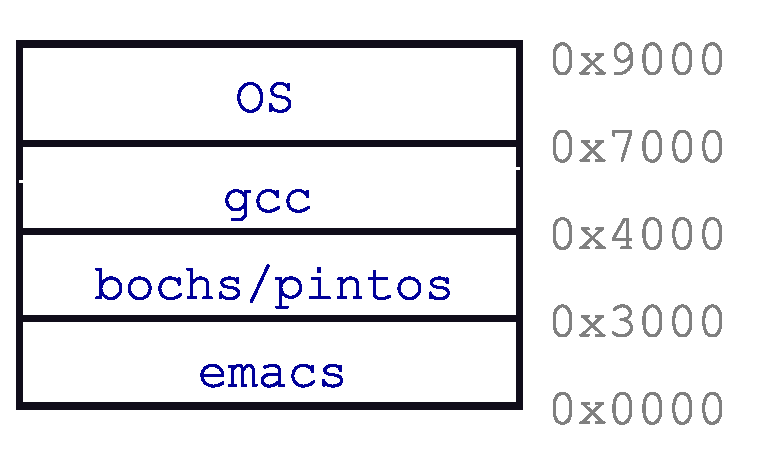
\includegraphics[height=1.5in]{figs/coexist}}

\medskip

\itms{
  \item Adressage direct
\ittms{
\item Que faire si gcc souhaite plus de mémoire ?
\item Si emacs souhaite 5 Go de mémoire sur une machine qui possède 4Go ?
\item Si gcc écrit par erreur sur l'adresse 0x7100 ?
\item Est-ce que le compilateur/linkeur doit savoir que gcc est à l'adresse 0x4000
?
\item Que faire si un processus veut libérer sa zone mémoire ?
  }
}
\end{slide}

\begin{slide}{Problèmes liés au partage de la mémoire physique}
\itms{
  \item \Red{Protection}
  \ittms{
    \item Un bug dans un processus peut corrompre un autre
    \item Protéger les écritures de $A$ dans la mémoire de $B$
    \item Protéger la lecture de la mémoire de $B$ (espionner mots de passe)
  (ssh-agent)
  }
  \item \Red{Transparence}
  \ittms{
    \item Un processus ne doit pas exiger des positions fixes en mémoire
  }
  \item \Red{Utilisation efficace de l'espace mémoire}
  \ittms{
    \item Mémoire totale des processus souvent dépasse la mémoire physique de la
    machine.
  }
}
\end{slide}

\begin{slide}{Mémoire Virtuelle}
\centerline{\includegraphics[width=112mm]{vmhilevel}}
\medskip


\itms{
  \item Chaque processus à son propre espace de mémoire ``virtuelle''
  \ittms{
    \item La MMU (Memory-Management Unit) traduit les adresses virtuelles en
    adresses physiques lors de chaque lecture ou écriture.
    \item L'application n'a jamais accès à la mémoire physique.
  }
  \item Protège l'accès à la mémoire
  \ittms{
    \item Un processus ne peut pas accéder à la mémoire d'un autre processus
  }
  \item La mémoire virtuelle peut dépasser la mémoire physique disponible
  \ittms{
    \item Pages non utilisées sont sauvegardées sur disque (swap)
  }
}
\end{slide}

\begin{slide}{Avantages de la mémoire virtuelle}
\itms{
  \item Supporte la migration dans l'espace mémoire
  \ittms{
    \item Une partie des pages est dans la RAM, une autre partie sur disque.
  }
  \item La majorité de la mémoire d'un processus est inactive (règle du 80/20).
  \ittms{
%\item[]\hspace*{-.3in}\includegraphics[width=4in]{figs/vmadv}
\item[]\hspace*{-.3in}\includegraphics[width=4in]{vmadv}
  \item Pages inactives sont sauvegardées sur disque
  \item D'autres processus peuvent récupérer la mémoire libérée
  \item Semblable à la virtualization CPU: processus n'utilise pas le CPU
  $\rightarrow$ préemption.
}
  \item Inconvénient: MV = indirection $\rightarrow$ ralentissement
}
\end{slide}

\begin{slide}{Idée 1: linkeur à la volée}
\centerline{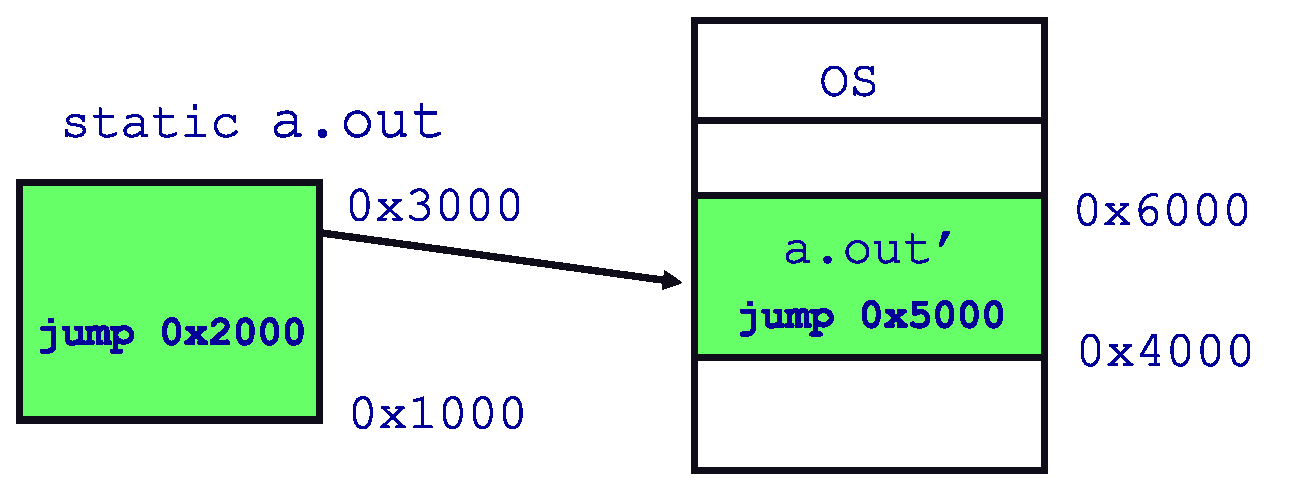
\includegraphics[height=1.3in]{figs/loadtime}}
\itms{
  \item \emph{Linkeur} patche les adresses des symboles
  \item Idée: fait le lien juste avant l'exécution (pas à la compilation)
  \ittms{
    \item Determine où les processus seront chargés (base)
    \item Ajuste toutes les adresses (par addition de la base)
  }
  \item Problèmes?
\pause
  \ittms{
    \item Comment mettre en place la protection ?
    \item Comment faire la migration (pointeurs) ?
    \item Nécessite un espace contigu suffisament grand.
  }
}
\end{slide}

\begin{slide}{Idée 2: registres base + borne}
\centerline{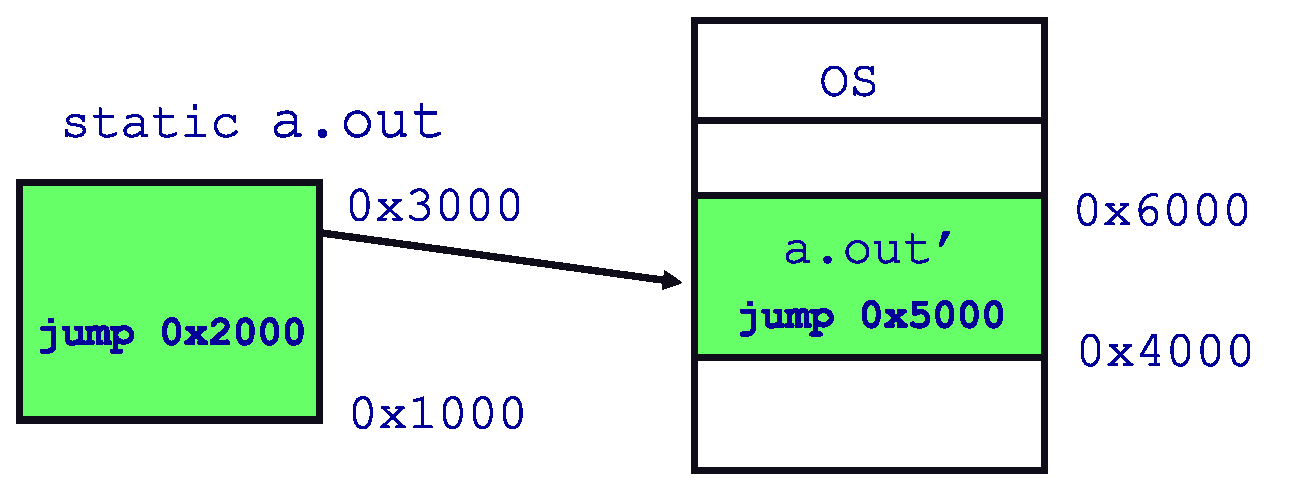
\includegraphics[height=1.3in]{figs/loadtime}}
\smallskip
\itms{
  \item Deux registres spéciaux:  \Red{base} et \Red{borne}
  \item Pour chaque écriture/lecture:
  \ittms{
    \item Adresse Physique = Adresse Virtuelle + \Red{base}
    \item On vérifie $0\le \mathrm{adr. virtuelle +
      \Red{base}}<\mathrm{\Red{borne}}$, sinon interruption.
  }
  \item Comment déplacer un processus en mémoire ?
  \ittms{
\onslide<2->{
    \item Change le registre \Red{base}
   }
  }
  \item Que faire lors d'un changement de contexte ?
  \ittms{
\onslide<3->{
    \item SE doit recharger les registres \Red{base} et \Red{borne}}
  }
}
\end{slide}

\begin{slide}{Définitions}
\itms{
  \item Les programmes écrivent sur des \Red{adresses virtuelles} (or \Red{logiques})
  \item La mémoire réelle utilise des \Red{adresses physiques} (ou \Red{réelles})
  \item Le matériel qui fait la traduction est la Memory Management Unit (\Red{MMU}) \\
  \ittms{
    \item[] 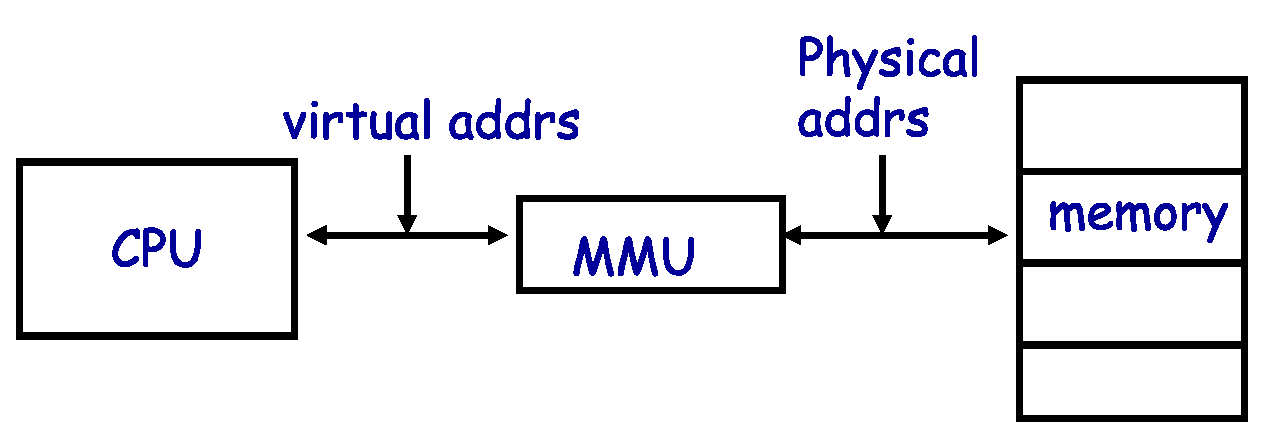
\includegraphics[width=96mm]{figs/mmu}
    \item Inclue dans le CPU
    \item Configurée en ring 0 (e.g., registres base et borne)
    \item Donne à chaque processus un \Red{espace d'adressage} virtuel.
  }
}
\end{slide}

\begin{slide}{Espace d'addressage}
\centerline{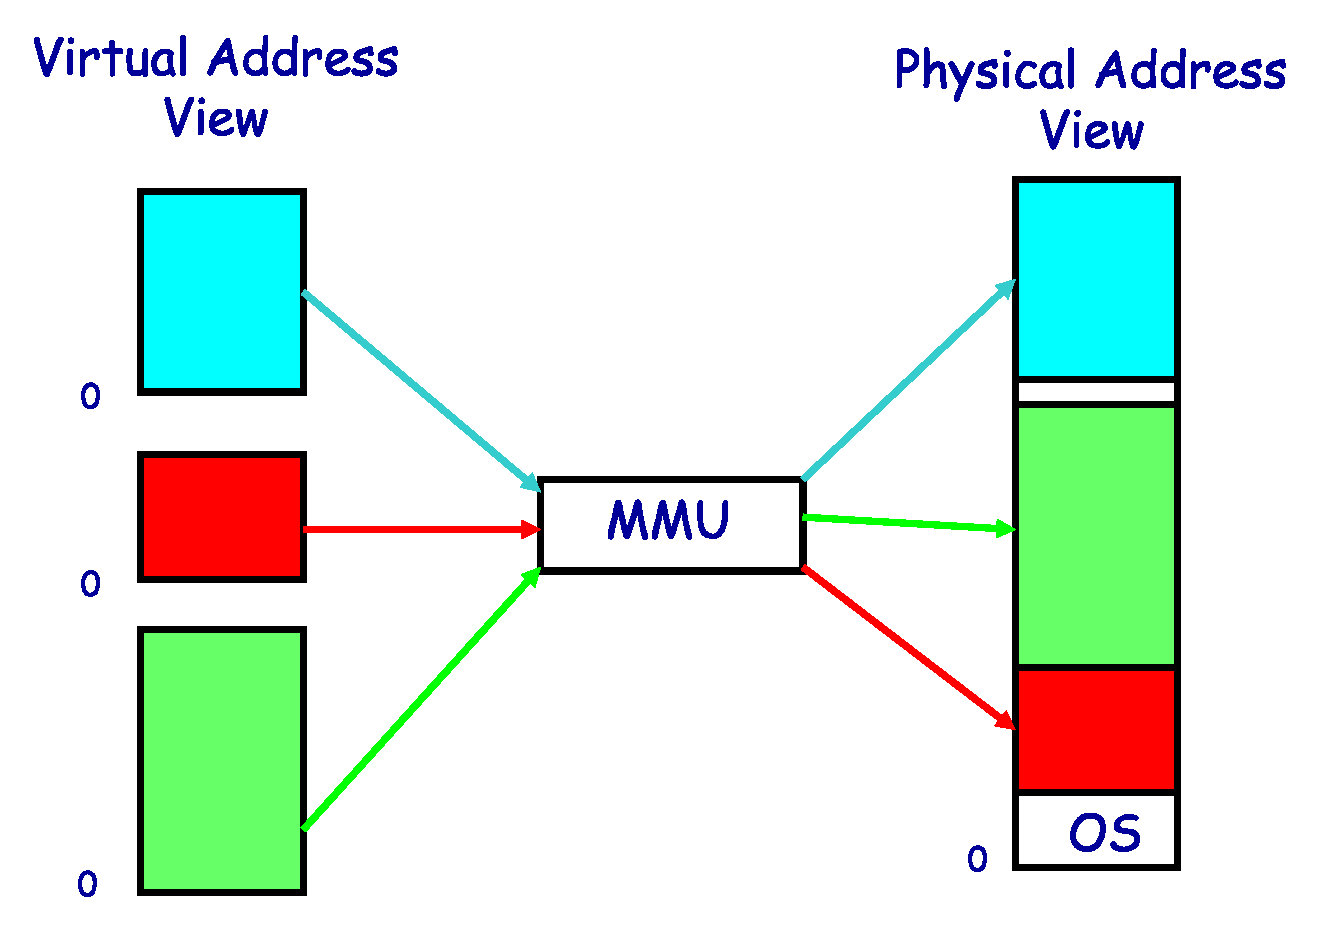
\includegraphics[width=4in]{figs/addressspace}}
\end{slide}

\begin{slide}{Avantages et Inconvénients du système Base+Borne}
\itms{
\item Avantages
\ittms{
  \item Matériel simple: 2 registres, un additionneur et un comparateur
  \item Rapide: quelques cycles seulement pour faire la traduction
  \item Exemple: Cray-1 utilisait un système Base + Borne
}
}
\begin{columns}[T,onlytextwidth]
\column{83mm}
\itms{
  \item Inconvénients
    \pause
  \ittms{
    \item La mémoire d'un processus doit être contigue
    \item Pas de mémoire partagée entre processus
  }
}
\column{25mm}
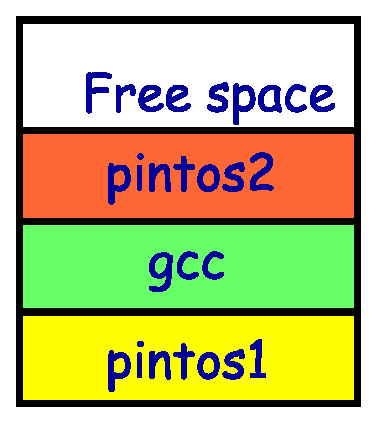
\includegraphics[width=25mm]{figs/bbtradeoff}
\end{columns}
\itms{
  \item Une solution:  segments multiples
  \ittms{
    \item E.g., on sépare le code, la pile et les données
    \item Eventuellement plusieurs segments de données
}}
\end{slide}

\begin{slide}{Segmentation}
\centerline{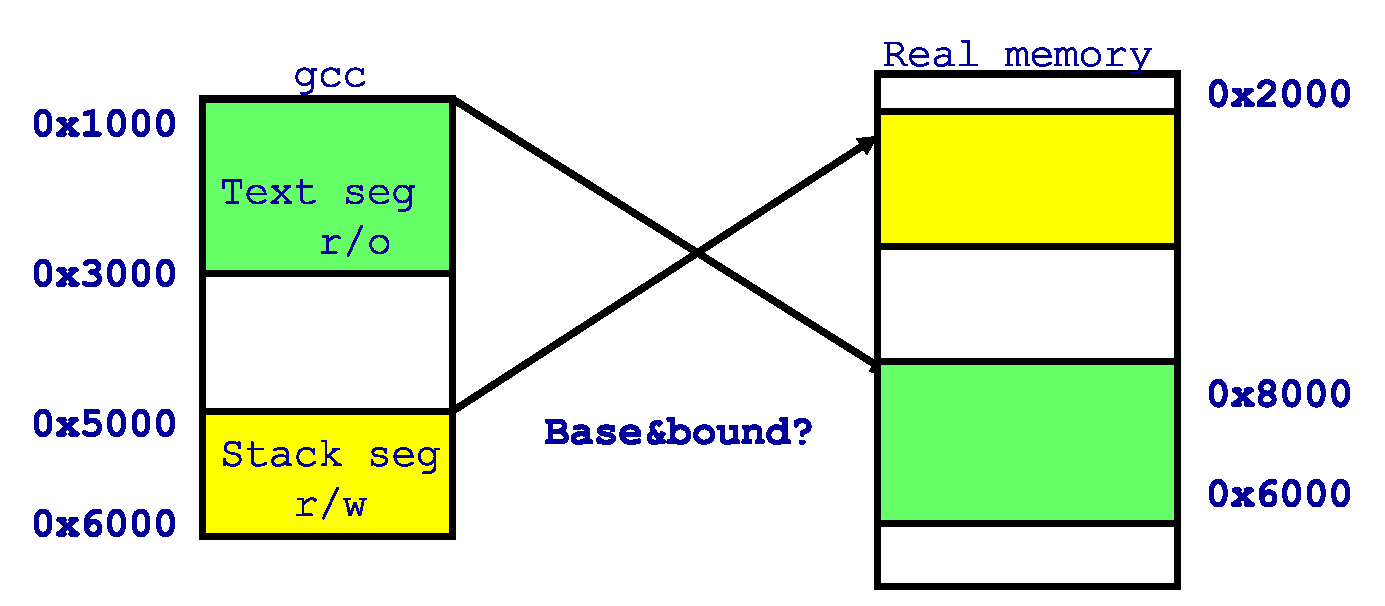
\includegraphics[height=2in]{figs/segmentation}}
\itms{
  \item Chaque processus dispose de plusieurs registres base/borne
  \ittms{
    \item Espace d'adressage dispose de plusieurs segments
    \item Protection mémoire par segment
  }
  \item Chaque accès mémoire doit spécifier le segment accédé
}
\end{slide}

\begin{slide}{Implémentation de la segmentation}
\centerline{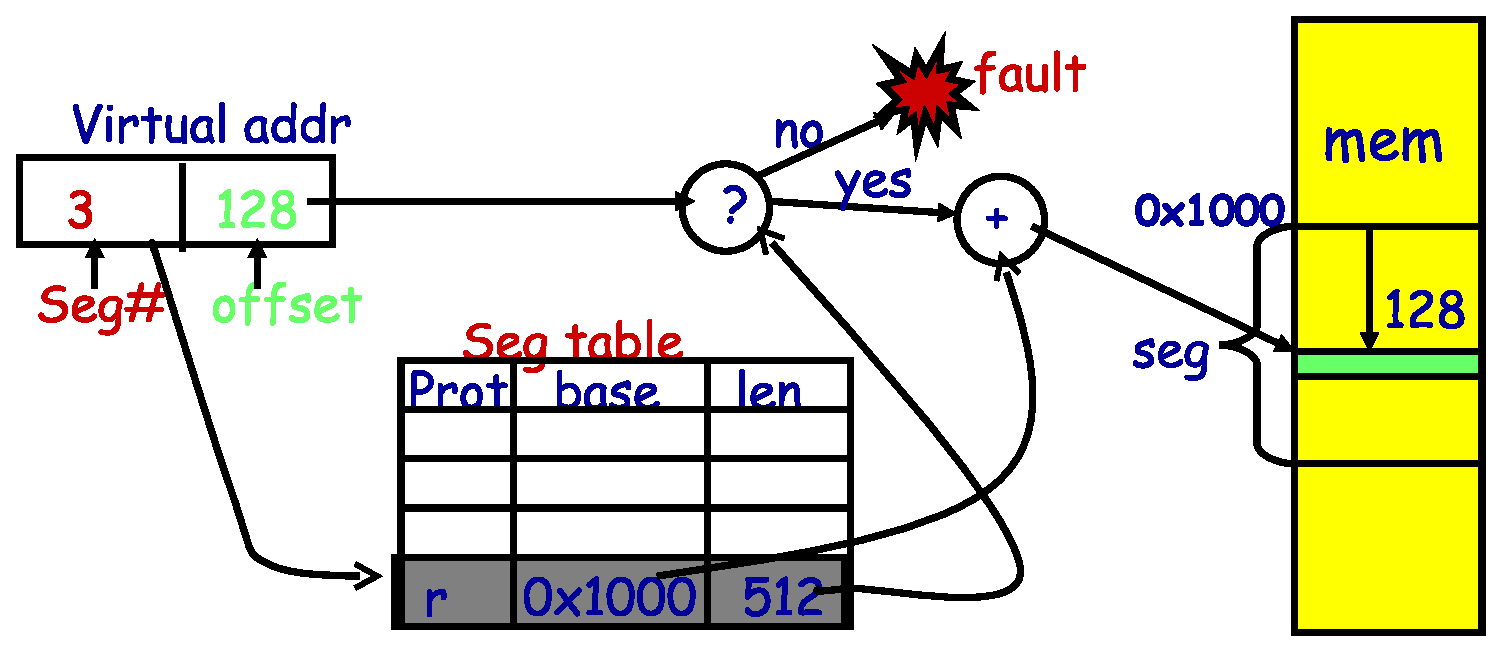
\includegraphics[height=2in]{figs/seg-mech}}
\itms{
\item Chaque processus dispose d'une table de segments
\item Chaque AV est composée d'un segment et d'un offset
\ittms{
  \item Bits de poids fort donnent le segment, Bits de poids faible donnent
  l'offset (PDP-10)
  \item Où alors segment choisi par l'instruction utilisée (x86)
}
}
\end{slide}

\begin{slide}{Exemple de Segmentation}
\centerline{\includegraphics[height=2.3in]{seg-example}}
\itms{
  \item Numéro de segment sur 4-bits (premier chiffre), offset sur 12 bits (3 derniers chiffres)
  \ittms{
    \item Où est 0x0240? 0x1108? 0x265c? 0x3002? 0x1600?
  }
}
\end{slide}

\begin{slide}{Avantages et Inconvénients de la segmentation}
\itms{
  \item Avantages
  \ittms{
    \item Plusieurs segments par processus
    \item Permet le partage (Comment ?)
    \item La mémoire du processus peut-être partiellement sur disque.
  }
}
\itms{
\item Inconvénients
\ittms{
  \item Surcoût d'accès à la table des segments
  \item Segments ne sont pas transparents pour le programme (instructions nécessaires pour choisir
  le segment)
  \item Segment de taille $n$ nécessite $n$ octets de mémoire \emph{contigue}
  \item Problème de \emph{Fragmentation}
}
}
\end{slide}

\begin{slide}{Fragmentation}
\vspace*{-.1in}
\itms{
\item \Red{Fragmentation} $\Longrightarrow$ Mémoire libre mais inutilisable
\item Après un certain temps:
\ittms{
  \item Segments de taille variable = plein de petits trous (fragmentation externe)
  \item Segments de taille fixe = pas de trous externes, mais segments
  sous-utilisés (fragmentation interne)
}
}
\centerline{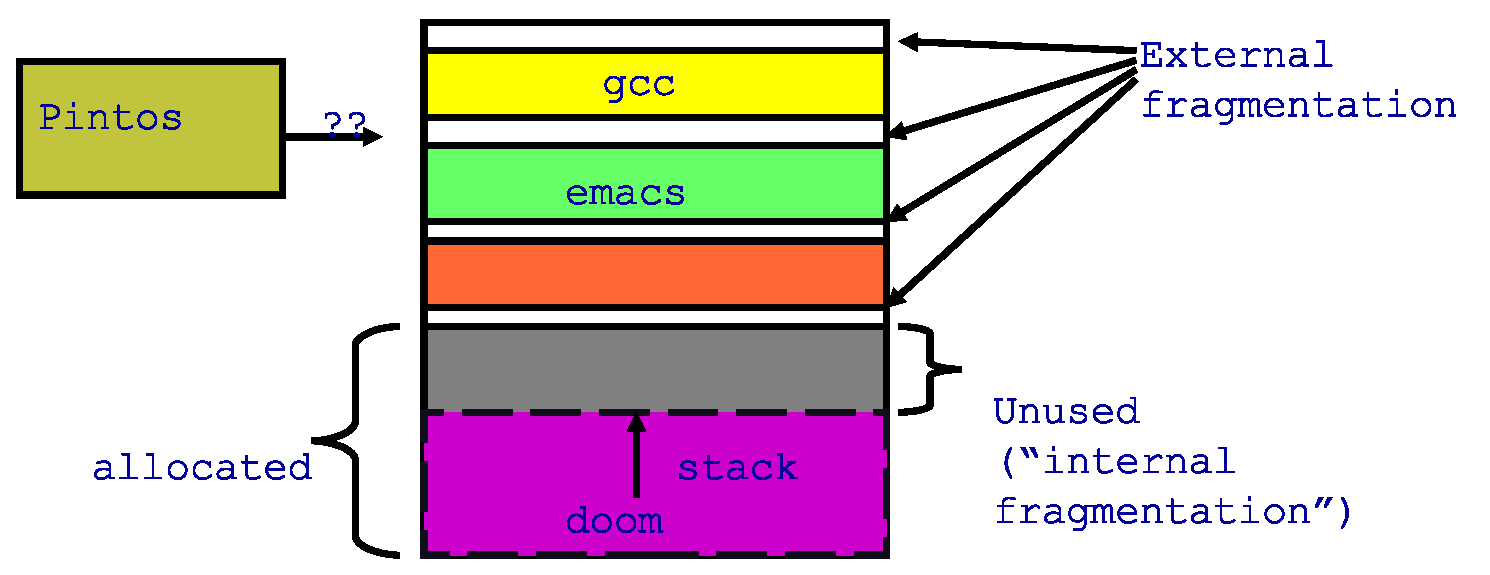
\includegraphics[width=4in]{figs/fragmentation}}
\end{slide}

\begin{slide}{Alternatives à la MMU}
\itms{
%  \item Segmentation
%  \ittms{
%    \item Part of each memory reference implicit in segment register\\
%	  $\mbox{segreg}\gets\langle\mathrm{offset,limit}\rangle$
%    \item By loading segment register code can be relocated
%    \item Can enforce protection by restricting segment register loads
%  }
  \item Protection au niveau du langage (Java)
  \ittms{
    \item Plusieurs modules se partagent le même espace d'adressage
    \item Le langage garantit l'isolation
  }
  \item Gardes générées au niveau du compilateur
  \ittms{
    \item Le compilateur émet des vérifications avant chaque écriture/lecture
    \item Google \href{http://code.google.com/p/nativeclient/}{Native Client}
          utilise cette méthode.
  }
}
\end{slide}

\begin{slide}{Pagination}
\itms{
  \item On divise la mémoire en petites pages (4K)
  \item Chaque page physique est associée à une page virtuelle
  \ittms{
    \item La table d'association est propre à chaque processus
  }
  \item Protection à la granularité d'une page
  \ittms{
    \item Page lecture seule (interruption)
    \item Page invalide (interruption)
    \item Le SE peut changer le mapping et revenir à l'application (chargement à
    la demande)
  }
}
\end{slide}

\begin{slide}{Avantages et Inconvénients de la pagination}
\centerline{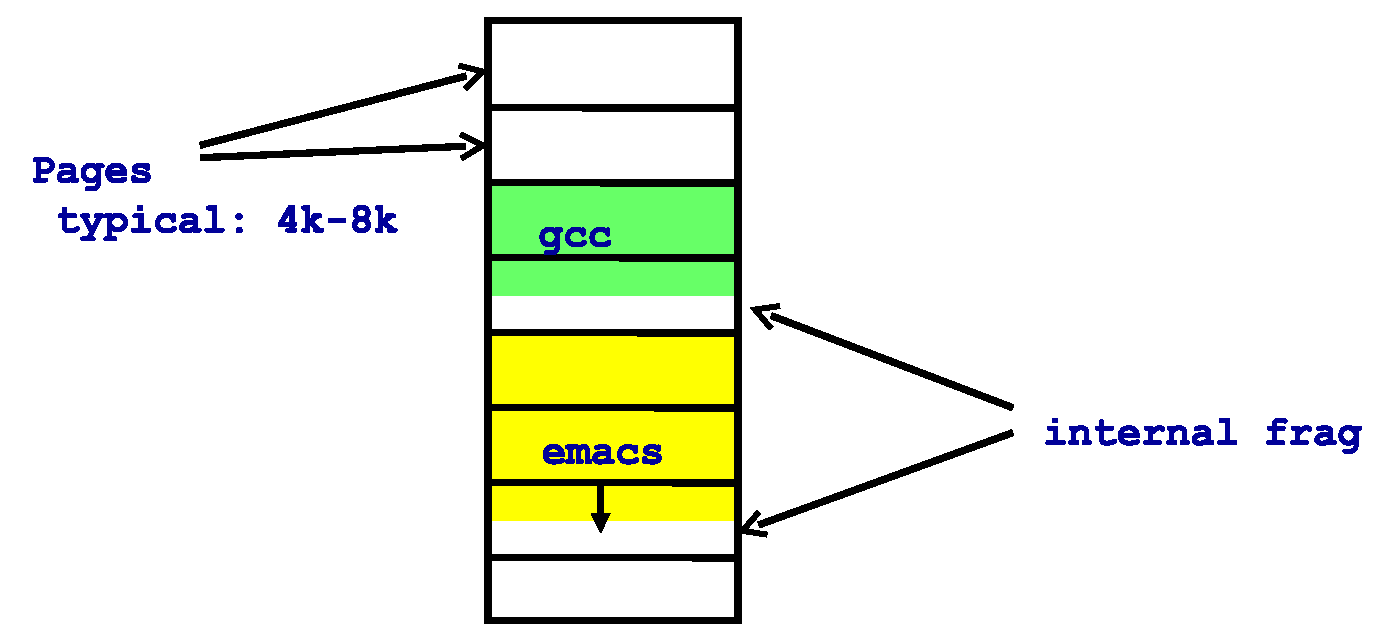
\includegraphics[width=4in]{figs/paging}}
\medskip
\itms{
  \item Pas de fragmentation externe
  \item Implémentation simple (allocation, free et swap). Les pages d'un même
  segment ne sont pas forcément contigues.
  \item En moyenne chaque segment mémoire gâche une demi page.
}
\end{slide}

\begin{slide}{Allocation simple}
\centerline{\input{paging}}
\itms{
  \item Alloue n'importe quelle page physique libre (pas forcément contigues)
  \item Les pages inactives peuvent être stockées sur disque
}
\end{slide}

\begin{slide}{Implémentation de la pagination}
\vspace*{-2mm}
\itms{
  \item Pages de taille fixe (souvent 4K)
  \ittms{
    \item 12 bits de poids faible ($\log_2$ 4K) pour l'offset
    \item bits de poids fort sont le numéro de page
  }
  \item Chaque processus possède une table des pages
  \ittms{
    \item Traduit les numéros de page virtuels en numéros de page physiques
    \item Des informations supplémentataires sur les protections, droits, etc.
  }
  \item Traduction = traduction du numéro de page + Offset}
\vspace*{-5mm}
\centerline{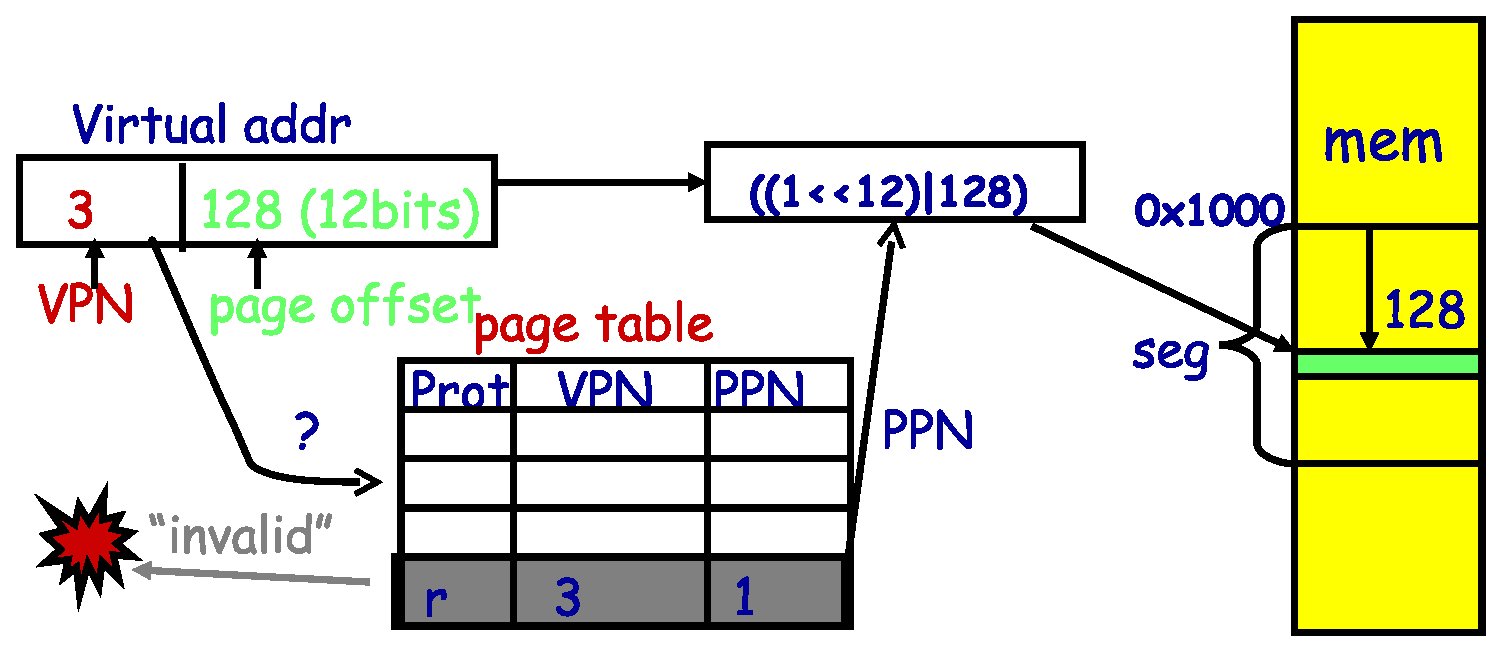
\includegraphics[width=4in]{figs/page-mech}}
\end{slide}

\begin{slide}{Quelle est la taille de la table des pages ?}
  \itms{
    \item Page de 4K
    \item Adresse sur 32 bits (4Go)
    \item Nombre de pages = $2^{32}/4096$ =  1.048.576
    \item Problème ?
    \pause
    \item Il faut plusieurs Mo pour stocker la table des pages de \emph{chaque processus}!
    \item \structure{Table des pages hiérarchique}
    }
\end{slide}

\begin{slide}{Pagination sur x86: table de pages hiérarchique}
\itms{
  \item Pagination activée grâce à un registre de controle (\texttt{\%cr0})
  \ittms{
    \item L'écriture de ce registre nécessite le mode privilégié
  }
  \item Souvent page 4K
  \item \texttt{\%cr3}: pointe vers le répertoire des tables

  \item Répertoire des tables: 1024 entrées
  \ittms{
    \item Chaque entrée pointe vers une table de pages
  }
  \item Table des pages: 1024 entrées
  \ittms{
    \item Chaque entrée donne la traduction d'une page de 4K
    \item Chaque table est donc en charge de 4Mo de mémoire virtuelle
  }
}
\end{slide}

\begin{slide}{Traduction sur x86}
\hspace*{-3mm}\input{x86.tex}
\end{slide}

\begin{slide}{Répertoire sur x86}
  \bigskip
\input{pde.tex}
\end{slide}

\begin{slide}{Table des pages sur x86}
\bigskip
\input{pte.tex}
\end{slide}

\begin{slide}{Segmentation sur x86}
\itms{
  \item L'architecture x86 supporte aussi la segmentation
  \ittms{
    \item base du segment + adresse = \emph{adresse linéaire}
    \item La traduction virtuelle s'effecture sur l'adresse linéaire
  }
  \item Deux niveaux de traduction et protection
  \item À quoi cela sert d'avoir segmentation + pagination ?
  \pause
  \item La plus part du temps à rien (Historique)
  \ittms{
    \item La plus part des SE configurent base = 0, borne =
      0xffffffff \\
  }
  \item Quelques applications de niche:
  \ittms{
    \item VMware utilise la segmentation pour detecter des erreurs sur la VM
    \item OpenBSD utilise la segmentation pour rendre la pile non executable
  }
}
\end{slide}

\begin{slide}{Coût de la Pagination: comment la rendre efficace ?}
\itms{
  \item Traduction sur x86 nécessite trois accès par lecture/ecriture:
  \ittms{
    \item Lecture de l'entrée dans le répertoire
    \item Lecture de l'entrée dans la table des pages
    \item Lecture de l'adresse initiale après traduction
  }
  \pause
  \item Pour être efficace le CPU cache les traductions récentes
  \ittms{
    \item \emph{Translation Lookaside Buffer} or \Red{TLB}
    \item Chaque TLB contient les dernières entrées de page accédées
    \item Configuration typique: 64-2K entrées, 4-way to fully associative, 95\% hit rate
  }
  \item Pour chaque accès
  \ittms{
    \item Si l'adresse est dans le TLB, traduction directe
    \item Sinon parcours du répertoire de pages et stockage dans le TLB pour les
    prochains accès\\
  }
}
\end{slide}

\begin{slide}{TLB details}
\itms{
\item TLB opère directement sur le pipeline CPU $\Longrightarrow$ rapide
\item Que se passe t'il lors d'un changement de contexte ?
\ittms{
  \item Flush TLB
  \item Chaque entrée est taggée avec un PID
}
\item C'est le rôle du SE de maintenir le TLB valide
\item E.g., x86 instruction \emph{invlpg}
  \ittms{
   \item Invalide une entrée TLB
  }
  }
\end{slide}

\begin{slide}{x86 long mode paging}
\vspace*{-6mm}
\hspace*{-4mm}\input{long.tex}
% \itms{
%   \item Why are aren't upper 16 bits of VA used?
% % Table walking is slow, would hurt performance
% }
\end{slide}

\begin{slide}{Espace d'adressage du SE}
\itms{
  \item Son propre espace ?
  \ittms{
    \item Impossible: sur de nombreus machines un appel système ne change pas les
    tables de pages
    \item Rendrai plus difficile le passage de pointeurs à un appel système
  }
  \item Donc OS dans le même espace d'adresse que le processus
  \ittms{
    \item Utilise la protection des pages pour protéger la zone mémoire du SE
  }
}
\end{slide}

\begin{slide}{Avantages de la pagination}
\itms{
  \item Chargement à la demande
  \item Augmenter la taille de la pile
  \item Allocation des pages BSS
  \item Données et bibliothèques partagées
  \item Pages partagées
  \item Copy-on-write (\texttt{fork}, \texttt{mmap}, etc.)
}
\end{slide}

\end{document}
